\header{
    \headtitle{La branleuse de taureau} \label{la-branleuse-de-taureau}
    %
    
    \insertComment{Chanson de Gérard Doulssane (1977).}{}
}
%
\enluminure{4}{\href{https://www.youtube.com/watch?v=zCt7jsMMdNc}{C}}{'est} la branleuse de taureaux,
\\Qui va, qui vient, qui fait son ouvrage.
\\C'est la branleuse de taureaux,
\\Qui va, qui vient, toujours au boulot.
\\\\Dans une ferme modèle, 
\\ Tape ta pine, pompe le noeud
\\Depuis qu'elle n'est plus pucelle, 
\\ Tape ta pine, pompe le noeud
\\Elle titille avec passion
\\ Tape ta pine, pompe le noeud
\\Pour faire l'insémination. 
\\ Tape ta pine, pompe le noeud
\\C'est elle qui tire la liqueur
\\ Tape ta pine, pompe le noeud
\\A ces beaux reproducteur
\\ Tape ta pine, pompe le noeud
\\Qui ont le gland aussi gros qu'un cocher
\\Et des glaouis comme des fesses.
\\Si, en suçant, elle avale la purée,
\\Elle est nourrie pour toute l'année.
\\\\Pomper la semence à ces  bestiaux,
\\C'est pas très sain, qu'elle a du courage!
\\Faut d'l'expérience et du brio:
\\Elle a la main, la branleuse de taureaux!
\breakpage
Pour arrondir ses fins d'mois, 
\\ Tape ta pine, pompe le noeud
\\Elle va tapiner au bois 
\\ Tape ta pine, pompe le noeud
\\Sa petite spécialité 
\\ Tape ta pine, pompe le noeud
\\Lui assure des habitués! 
\\ Tape ta pine, pompe le noeud
\\On vient la voir de très loin 
\\ Tape ta pine, pompe le noeud
\\Avec la pine à la main. 
\\ Tape ta pine, pompe le noeud
\\Mais elle se marre devant les vits bandés
\\Sous l'effet de ses caresses,
\\Quand elle compare avec ses bovidés:
\\C'est des cure dents pour les pigmés !
\begin{figure}[h!]
\centering
   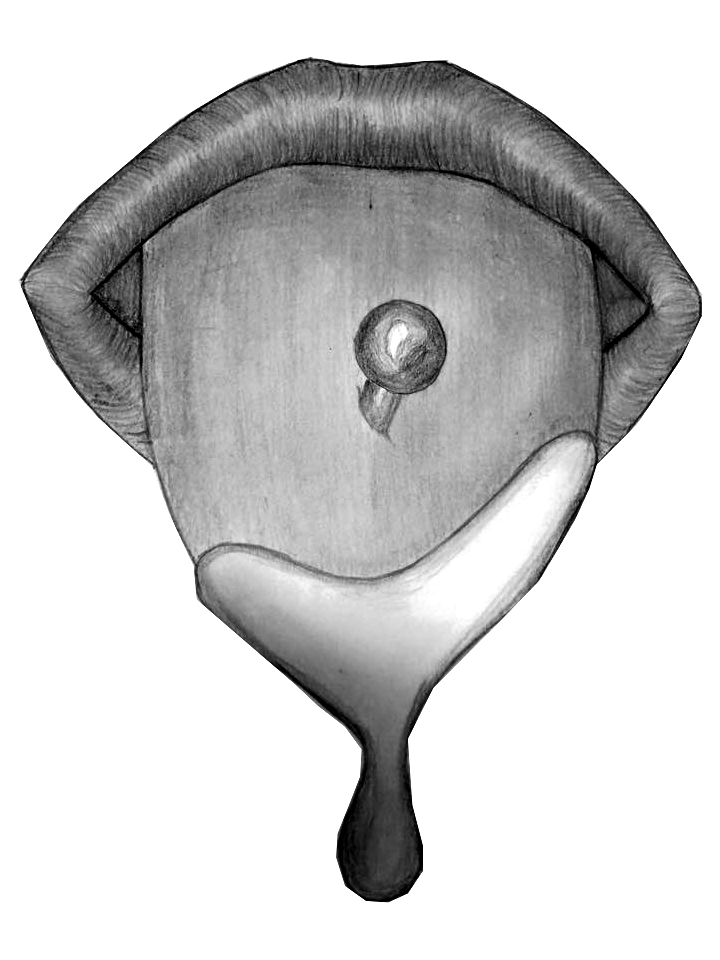
\includegraphics[width=0.62\textwidth]{images/taureau.png}
 \end{figure}
 
 \breakpage